\section{Sizing and Gating: Supplementary Derivations}
\label{sec:appendix-sizing-gating}

This section provides supplementary derivations and empirical evidence for \S\ref{sec:eval-dedrift}. The Sizing portion covers the theoretical derivation of scaling laws (\S\ref{sec:appendix-sizing-derivation}), sources and quantitative bounds of negative bias (\S\ref{sec:appendix-sizing-bias}), and stability evidence for accuracy across a wider parameter range (\S\ref{sec:appendix-sizing-supp}). The Gating portion covers metric selection and semantic validation (\S\ref{sec:appendix-gating-metric}), the scale separation of $K_{\text{eff}}/L$ and theoretical analysis of the occupancy threshold (\S\ref{sec:appendix-gating-separation}), and the necessity argument for the three-state design (\S\ref{sec:appendix-gating-tristate}).

\subsection{Fusion Law and Variance Scaling}
\label{sec:appendix-sizing-derivation}

This section supplements the derivations of two key phenomena: first, why multi-view fusion yields a $1/\sqrt{V}$ variance reduction; second, why the de-drift term eliminates the influence of $q$ in expectation under drift conditions, along with an approximate variance scaling that aids understanding of the $m_0$/$V$ scaling laws.

\subsubsection{Theoretical Derivation of the Fusion Law}
\label{sec:appendix-fusion-law}

The multi-view fusion law ($\text{Std} \propto 1/\sqrt{V}$) follows from the basic property of averaging independent estimators. Let the sizing estimates $\hat D_v$ from each view be independent and identically distributed with common variance $\text{Var}(\hat D_v) = \sigma^2$. The fused estimate is:
\[
\hat D = \frac{1}{V}\sum_{v=1}^{V} \hat D_v.
\]
By independence, the variance of the fused estimate is $\text{Var}(\hat D)=\sigma^2/V$, so $\text{Std}(\hat D) = \sigma/\sqrt{V} \propto V^{-0.5}$. In log-log coordinates, $\log(\text{Std}) = \text{const} - 0.5 \cdot \log(V)$, i.e., the slope is $-0.5$.

We now derive the expectation and variance of the de-drift statistic itself, to explain both drift invariance and accuracy scaling laws (\S\ref{sec:eval-dedrift}).

Let $M=L\cdot m_0$ denote the total cell count of a single view. In implementation, each diff key updates only $k$ distinct positions among the $W\cdot m_0$ candidate cells within the window of its corresponding segment; here we adopt a marginal distribution approximation where, after uniform hashing of window start positions on the section axis, these updates are treated as landing on $k$ distinct positions among the global $M$ cells, yielding an interpretable closed form (the main text \S\ref{sec:dedrift} discusses the applicability and boundaries of this approximation). The symmetric difference contains $D$ diff keys in total. Each diff key produces a sign $\sigma_i\in\{+1,-1\}$, where $\Pr(\sigma_i=+1)=q$. Let $X_{ij}\in\{0,1\}$ indicate whether the $i$-th key hits the $j$-th cell; then the cell count is:
\[
C_j=\sum_{i=1}^{D}\sigma_i X_{ij}.
\]
Define the global aggregate statistics:
\[
S_{\text{net}}=\sum_{j=1}^{M}C_j,\qquad
S_{\text{sq}}=\sum_{j=1}^{M}C_j^2.
\]
Expanding the square and summing over $j$:
\[
S_{\text{sq}}=\sum_{j}\sum_{i}\sigma_i^2 X_{ij}+\sum_{j}\sum_{i\neq \ell}\sigma_i\sigma_\ell X_{ij}X_{\ell j}.
\]
In the first term, $\sigma_i^2\equiv 1$, and each key hits $k$ cells, so:
\[
\mathbb{E}\left[\sum_{j}\sum_{i}\sigma_i^2 X_{ij}\right]=Dk.
\]
In the second term, $\mathbb{E}[\sigma_i\sigma_\ell]=\mathbb{E}[\sigma_i]\mathbb{E}[\sigma_\ell]=(2q-1)^2$, and for two distinct keys, the expected size of the intersection of their $k$-element landing sets is approximately $k^2/M$ (note: fixing the first key's $k$ cells, the probability that any one cell is hit by the second key is approximately $k/M$; summing over the $k$ cells gives expected intersection $\approx k\cdot(k/M)$), so:
\[
\mathbb{E}\left[\sum_{j}\sum_{i\neq \ell}\sigma_i\sigma_\ell X_{ij}X_{\ell j}\right]\approx D(D-1)(2q-1)^2\cdot \frac{k^2}{M}.
\]

On the other hand, note that $S_{\text{net}}=\sum_j C_j=\sum_i \sigma_i\sum_j X_{ij}=k\sum_i \sigma_i$, so:
\[
\mathbb{E}[S_{\text{net}}^2]=k^2\cdot \mathbb{E}\!\left[\left(\sum_i \sigma_i\right)^2\right]
=k^2\left(D + D(D-1)(2q-1)^2\right).
\]

Therefore:
\begin{align*}
\mathbb{E}\!\left[S_{\text{sq}}-\frac{S_{\text{net}}^2}{M}\right]
&\approx Dk + D(D-1)(2q-1)^2\frac{k^2}{M} \\
&\quad -\frac{k^2}{M}\left(D + D(D-1)(2q-1)^2\right) \\
&= Dk\left(1-\frac{k}{M}\right).
\end{align*}


This result has two implications. First, the $(2q-1)^2$ terms cancel exactly after de-drifting, so \textbf{the expectation does not depend on $q$}. This is why the de-drifted statistic remains stable under side imbalance in the main-text experiments (\S\ref{sec:eval-dedrift}). Second, $1-k/M$ reflects the energy dilution from cross-key collisions in the finite cell space, consistent with the $(1-k/M)$ term in the sizing denominator used in implementation.

This derivation uses the global quantity $S_{\text{sq}}-S_{\text{net}}^2/M$, whereas the experiments use the per-section form $\sum_s E_s$. The two differ by a small constant-factor term that diminishes as $m_0$ increases, but the core conclusion---that the expectation does not depend on $q$---holds for both definitions.

\paragraph{Bessel Correction (Degrees-of-Freedom Correction)}
In implementation, $E_s=\sum_{j=1}^{m_0}(\Delta_j-\bar{\Delta}_s)^2$ is equivalent to the unnormalized sample variance of the $m_0$ cell counts within section $s$. By the degrees-of-freedom identity,
\[
\mathbb{E}[E_s]=(m_0-1)\cdot \mathrm{Var}(\Delta_j\mid \text{section }s),
\]
so when the target quantity is written at the scale of $m_0 \mathrm{Var}(\cdot)$, the estimator based on $\sum_s E_s$ carries a first-order multiplicative bias of $(m_0-1)/m_0$. Multiplying the sizing output by $m_0/(m_0-1)$ eliminates this bias---this is precisely the Bessel correction factor used in the main text and evaluation.

\subsubsection{Zero Energy and Skip Signal}
\label{sec:appendix-sizing-zero-energy}

By definition, $E_s=\sum_{j=1}^{m_0}(\Delta_j-\bar{\Delta}_s)^2\ge 0$, with $E_s=0$ if and only if all cell difference counts $\Delta_j$ within section $s$ are identical.
If $\mathrm{net\_sum}_s=\sum_j \Delta_j=0$ also holds, then $\Delta_j\equiv 0$, so section $s$ carries zero differential observation.

This section-level fact lifts to a segment-level skip criterion. For a segment $p$, let $W_v(p)$ denote its mapped width-$W$ section window in view $v$. If all sections in $W_v(p)$ satisfy both $E_s^{(v)}{=}0$ and $\mathrm{net\_sum}_s^{(v)}{=}0$ for any single view $v$, then every probe cell reachable from segment $p$ in that view is zero. Because any diff key belonging to $p$ would update $k\ge 1$ cells within $W_v(p)$, the zero observation implies that no such key exists---or that its contributions are exactly canceled by collisions from other segments, an event whose probability is negligible under random hashing and non-adversarial inputs.

The segment can therefore be excluded from downstream verification. Requiring the condition to hold across all $V$ views provides a strictly stronger guarantee.


\subsubsection{Variance Scaling and Poisson Approximation}

To provide an interpretable scaling, we use a common Poisson approximation: treating the load on each cell as approximately independent and with $\mathbb{E}[C_j^2]$ at the scale determined by $\lambda=Dk/M$. Under this approximation, $S_{\text{sq}}-S_{\text{net}}^2/M$ is approximately the sum of squares of $M$ nearly independent terms, whose leading variance term (analogous to the $\mathrm{Var}=2n$ property of the $\chi^2$ distribution) can be written as:
\[
\mathrm{Var}\!\left(S_{\text{sq}}-\frac{S_{\text{net}}^2}{M}\right)
\approx 2M\lambda^2
=2\cdot \frac{(Dk)^2}{M}.
\]

The mean is $\mathbb{E}[\cdot]\approx Dk(1-k/M)\approx Dk$, so the relative standard deviation under a single view satisfies:
\[
\mathrm{Std}(\mathrm{rel\_err})=\frac{\mathrm{Std}(\hat D)}{D}
\approx \Theta\!\left(\sqrt{\frac{1}{M}}\right)
=\Theta\!\left(\sqrt{\frac{1}{L\cdot m_0}}\right),
\]
and after independently averaging over $V$ views, further yields the $1/\sqrt{V}$ scaling:
\[
\mathrm{Std}(\mathrm{rel\_err}_{\text{fusion}})\approx \Theta\!\left(\sqrt{\frac{1}{V\cdot L\cdot m_0}}\right).
\]

This approximation accounts for three trends observed in the sizing subsection (\S\ref{sec:eval-dedrift}): increasing $V$ provides a predictable $1/\sqrt{V}$ variance reduction; increasing $m_0$ reduces error but with diminishing returns; and relative error depends only weakly on $D$ (the leading term in $D$ cancels).

The Poisson approximation is used to explain scaling slopes: with typical parameters $(V=4, L=2048, m_0=32)$, the approximation gives $\mathrm{Std}(\mathrm{rel\_err})$ of about 0.28\%, while the experimental observation is about 2.25\%; however, the scaling slopes in $V$ and $m_0$ remain consistent.

\subsection{Locality Bias of Sizing}
\label{sec:appendix-sizing-bias}

The sizing estimator $\hat{D} = \sum_s E_s/[k(1-k/M)]$ in \S\ref{sec:dedrift} uses the global pool $M = L \cdot m_0$ in its denominator. This is the marginal distribution approximation obtained by treating window start positions as uniformly hashed on the section axis: when differing keys are distributed across multiple segments, cross-window pairings dominate, and the approximation is reasonable. However, when differences are highly concentrated in a few segments, each key's hash landing points are strictly confined to the $W$ sections (a total of $M_{\text{local}} = W \cdot m_0$ cells) within its segment's window, and the effective collision pool shrinks to the local scale. In this case, the estimator's expectation satisfies
\[
\mathbb{E}[\hat{D}] \;\approx\; D \cdot \frac{1 - k/M_{\text{local}}}{1 - k/M} \;<\; D,
\]
i.e., the global approximation $(1{-}k/M)$ underestimates the intensity of local collisions, causing systematic underestimation. The magnitude of the bias is determined by the gap between $M_{\text{local}}$ and $M$: with typical parameters ($k{=}2$, $W{=}4$, $m_0{=}32$, $L{=}2048$), $M_{\text{local}}{=}128$, $M{=}65{,}536$, and the formula above gives a negative bias upper bound of approximately $1.6\%$. This bias decreases as $W/L$ shrinks---when differences are distributed across multiple segments or $L$ is large, the effective pool approaches the global $M$, and the bias approaches zero. The main conclusion from \S\ref{sec:appendix-sizing-derivation}---that the expectation does not depend on $q$---is unaffected by this approximation.

In experiments, one can observe that the negative bias is more pronounced when $m_0$ is small (because $k/M_{\text{local}}$ is larger), and converges rapidly as $m_0$ increases (Figure~\ref{fig:c3-a2}). If explicit compensation is desired, $M_{\text{local}}$ can replace $M$ in the denominator; however, at typical deployment parameters, the 1.6\% bias magnitude usually does not have operational impact.


\subsection{Supplementary Empirical Evidence for Sizing Accuracy}
\label{sec:appendix-sizing-supp}

\paragraph{Baseline evidence under the standard setting}
For sizing, the principal accuracy metric in the main text is
$\mathrm{Std(rel\_err)}$. This section provides the additional
per-setting statistics, broader parameter sweeps, and
supporting evidence underlying the sizing results. The main
text \S\ref{sec:eval-dedrift} established three scaling laws:
the fusion law ($\mathrm{Std} \propto V^{-0.5}$), the
accuracy-memory trade-off of $m_0$, and the weak dependence of
relative error on discrepancy size $D$. We first revisit the
fusion law under the baseline configuration. Across the
parameter grid summarized in Figure~\ref{fig:c3-a1}, log-log
regression of $\mathrm{Std(rel\_err)}$ against $V$ yields a
mean slope of $-0.498$ (std.\ 0.050), close to the theoretical
value $-0.5$; Table~\ref{tab:c3-1} lists representative values
showing the corresponding decrease in relative error standard
deviation as $V$ increases. The third law is an implicit
prerequisite for the first two---if relative error drifted
significantly with $D$,
the promise of predictable accuracy from a fixed memory budget would no longer hold. This section therefore verifies the robustness of all three laws under two parameter settings.

\begin{table}[!htbp]
\centering
\small
\begin{tabular}{rccccc}
\toprule
$V$ & 1 & 2 & 4 & 8 & 16 \\
\midrule
\texttt{Std(rel\_err)} (\%) & 3.53 & 2.66 & 2.25 & 1.33 & 1.01 \\
\bottomrule
\end{tabular}
\caption{Fusion law under a representative configuration ($m_0{=}32,\ L{=}2048$).}
\label{tab:c3-1}
\end{table}

\begin{figure}[!htbp]
\centering
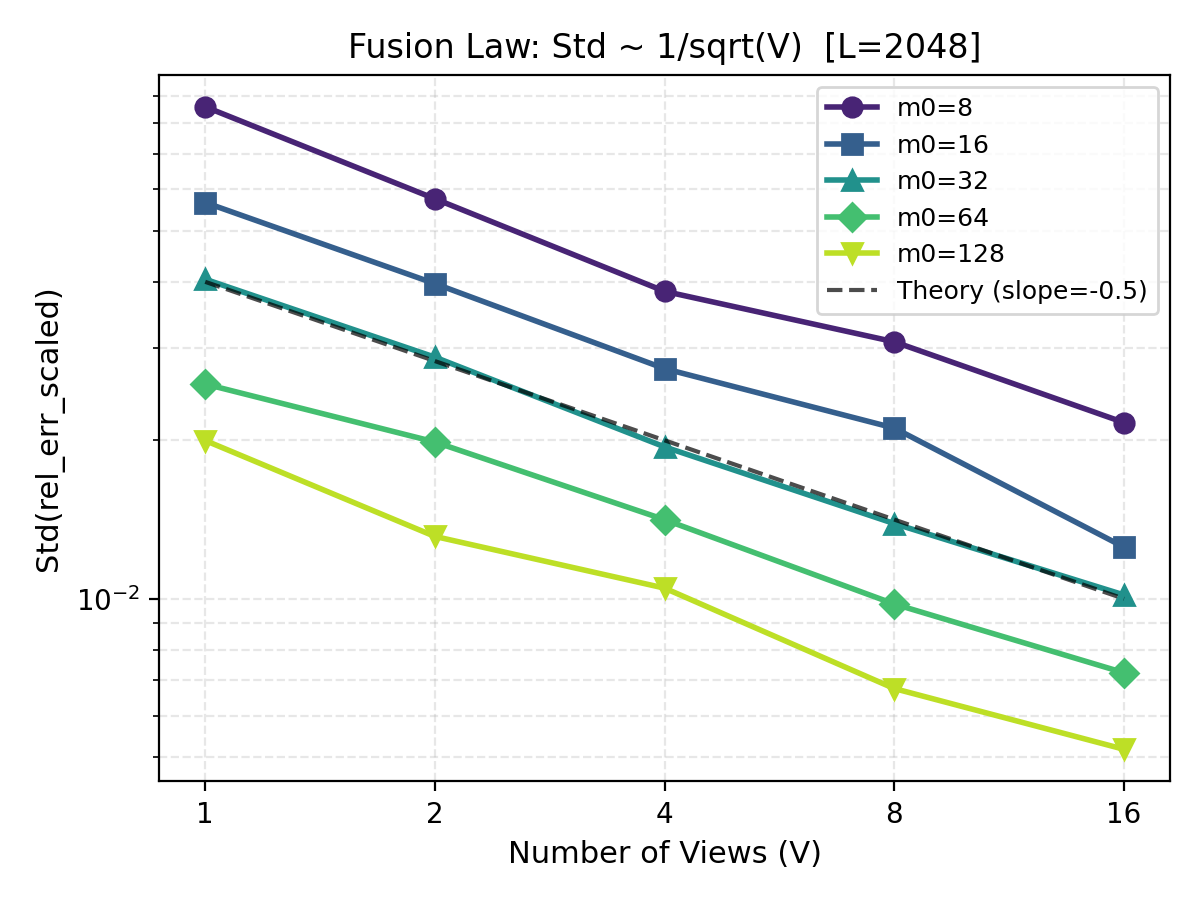
\includegraphics[width=0.9\linewidth]{figures/exp04v2_fusion_law.png}
\caption{Empirical verification of the fusion law: across a parameter grid covering 90 $(m_0, L, D)$ configurations, the mean log-log slope is $-0.498$, in close agreement with the theoretical prediction of $-0.5$.}
\label{fig:c3-a1}
\end{figure}

\begin{figure}[!htbp]
\centering
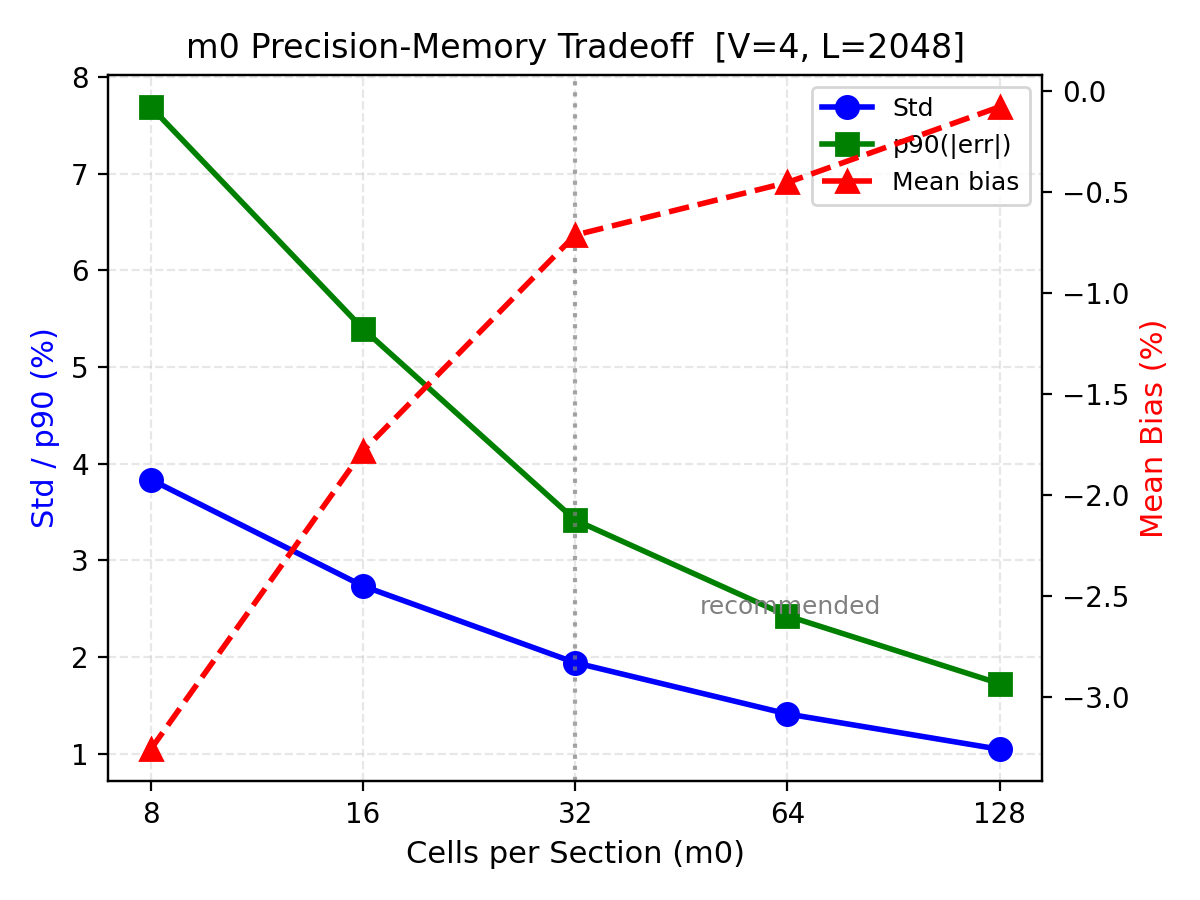
\includegraphics[width=0.9\linewidth]{figures/exp04v2_m0_tradeoff.png}
\caption{Accuracy-memory trade-off of $m_0$: $\mathrm{Std(rel\_err)}$ decreases monotonically with $m_0$, with diminishing returns beyond $m_0=32$; the negative bias converges simultaneously.}
\label{fig:c3-a2}
\end{figure}


\paragraph{Robustness under a more demanding setting}
Under the baseline configuration ($V \in \{1,2,4,8,16\}$, $m_0 \in \{8,\ldots,128\}$, $L \in \{1024,\ldots,4096\}$), as $D$ spans from $10^2$ to $10^7$, the \texttt{Std(rel\_err)} aggregated across all $(V,m_0,L)$ fluctuates around 2\%, indicating that relative accuracy is primarily governed by probe capacity parameters rather than discrepancy magnitude (Figure~\ref{fig:c3-a3}).
Additionally, we repeated the verification under a more demanding system and fault configuration:
larger scale $P{=}10^6$, higher fault density $B{=}100$, stronger asymmetry ($q=0.1$), and lighter updates ($W{=}2, k{=}1$).
Under this stress setting, all three laws are reproduced. For the fusion law, log-log regression over $(L,m_0,D)$ combinations for $V\in\{1,4,16\}$ yields a mean slope of approximately \textbf{-0.489} (median \textbf{-0.494}), consistent with the theoretical $-0.5$ (Figure~\ref{fig:c3-a4}).
The accuracy-memory trade-off of $m_0$ likewise holds: the aggregated \texttt{Std(rel\_err\_scaled)} decreases monotonically with $m_0$ and exhibits diminishing returns (Figure~\ref{fig:c3-a5}). And the weak dependence on $D$ continues to hold over a larger span: as $D$ ranges from $10^3$ to $10^8$, no order-of-magnitude deterioration in relative error is observed.

\begin{figure}[!htbp]
\centering
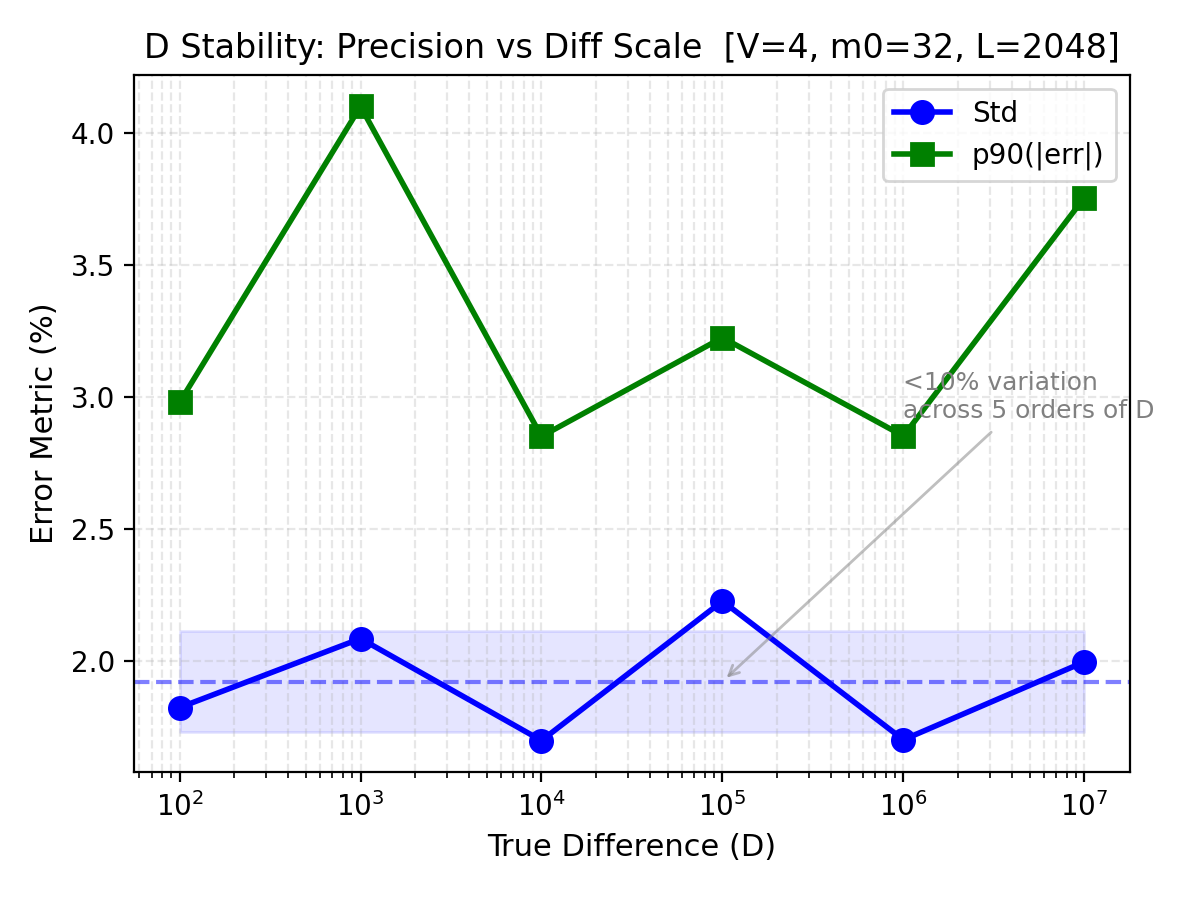
\includegraphics[width=0.9\linewidth]{figures/exp04v2_D_stability.png}
\caption{Weak dependence of sizing relative accuracy on $D$: as $D$ varies across multiple orders of magnitude, the relative error metrics show only modest fluctuation overall.}
\label{fig:c3-a3}
\end{figure}

\begin{figure}[!htbp]
\centering
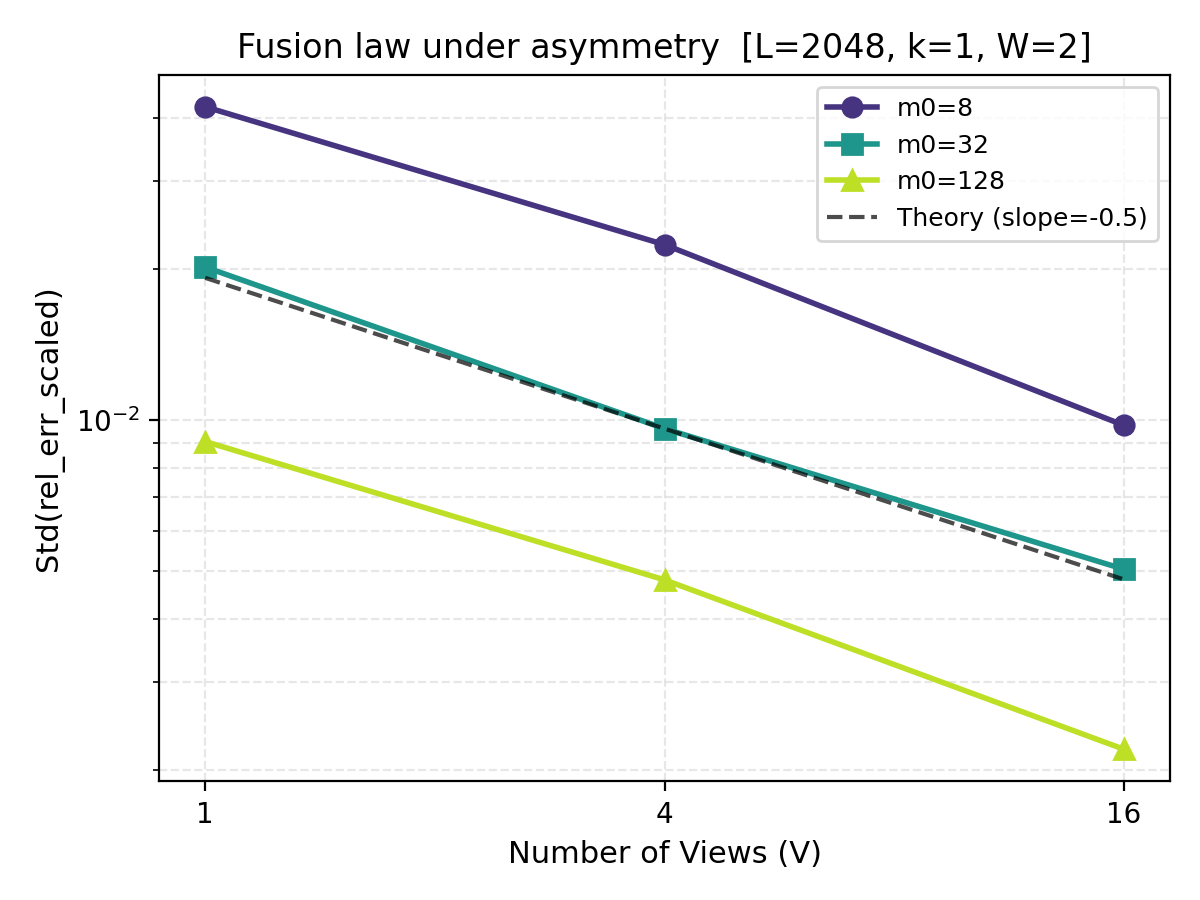
\includegraphics[width=0.9\linewidth]{figures/exp04v3_fusion_law.png}
\caption{Reproduction of the fusion law under a more demanding setting: mean log-log slope approximately $-0.489$, consistent with the theoretical $-0.5$.}
\label{fig:c3-a4}
\end{figure}

\begin{figure}[!htbp]
\centering
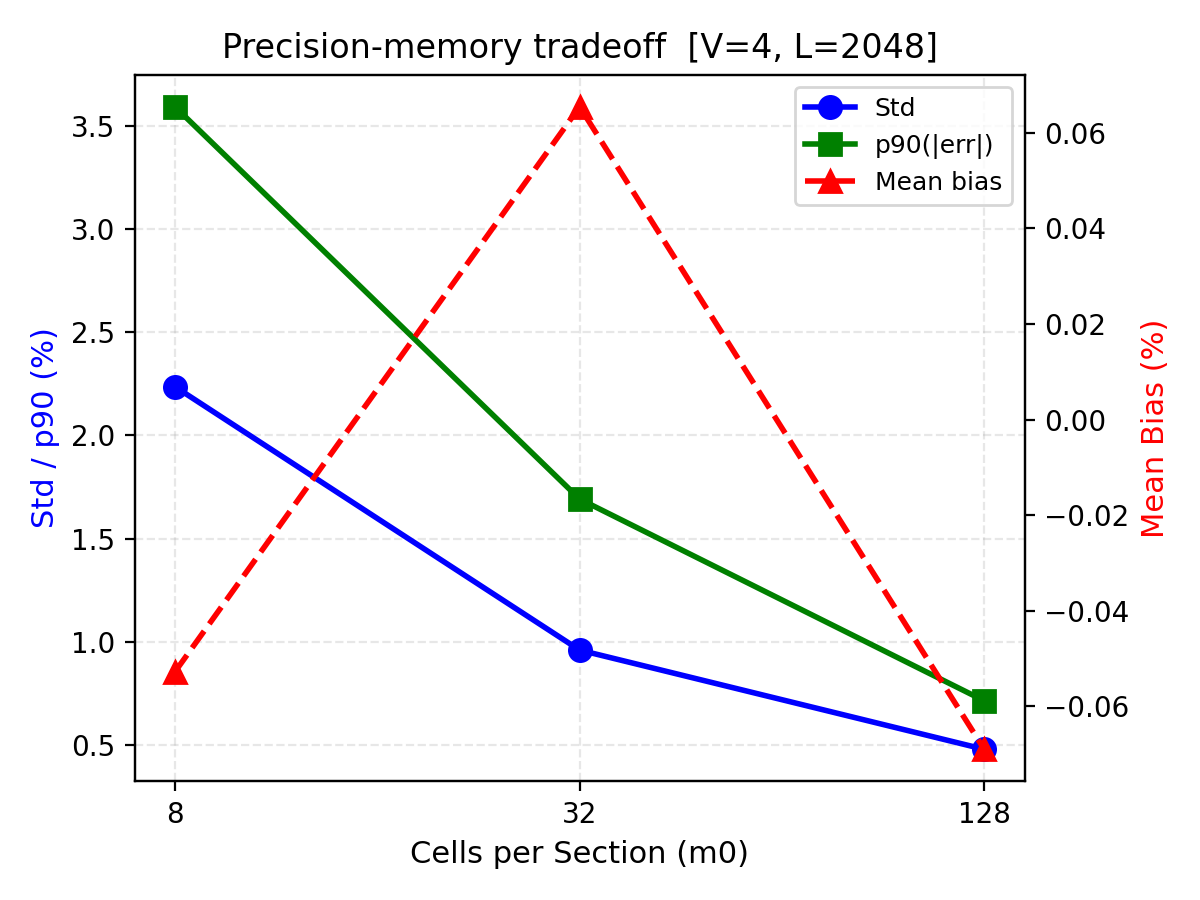
\includegraphics[width=0.9\linewidth]{figures/exp04v3_m0_tradeoff.png}
\caption{Reproduction of the $m_0$ accuracy-memory trade-off under a more demanding setting. Unlike the baseline configuration (Figure~\ref{fig:c3-a2}), after Bessel correction the mean bias has dropped to within 0.06\% and fluctuates around zero.}
\label{fig:c3-a5}
\end{figure}



\subsection{Metric Selection and Semantic Validity for Gating}
\label{sec:appendix-gating-metric}

\paragraph{Separability of candidate metrics}
Gating requires a scalar metric to quantify the concentration of the energy spectrum (\S\ref{sec:gating}). Before settling on $K_{\text{eff}}/L$, we compared four candidate statistics across a sweep covering bimodal ($B\in\{1,5,10,50,200\}$), diffuse ($D=10^5$), and heavy\_share
workloads over multiple $(P,L)$ configurations (with $V{=}2$, $m_0{=}16$, $W{=}4$, $k{=}2$; 50 repetitions per group): $K_{\text{eff}}/L$, Top-1/32
energy share, Gini coefficient, and normalized entropy. As shown in Figure~\ref{fig:c3-b1}, $K_{\text{eff}}/L$ exhibits the largest separation between bimodal and diffuse (medians differ by approximately 36$\times$), and this separation remains stable across different $(P,L)$ configurations.
Furthermore, $K_{\text{eff}}/L$, based on the continuous definition of the Herfindahl index, serves as a continuous measure of spatial concentration without relying on discrete binning or top-$k$ truncation.


\begin{figure}[!htbp]
\centering
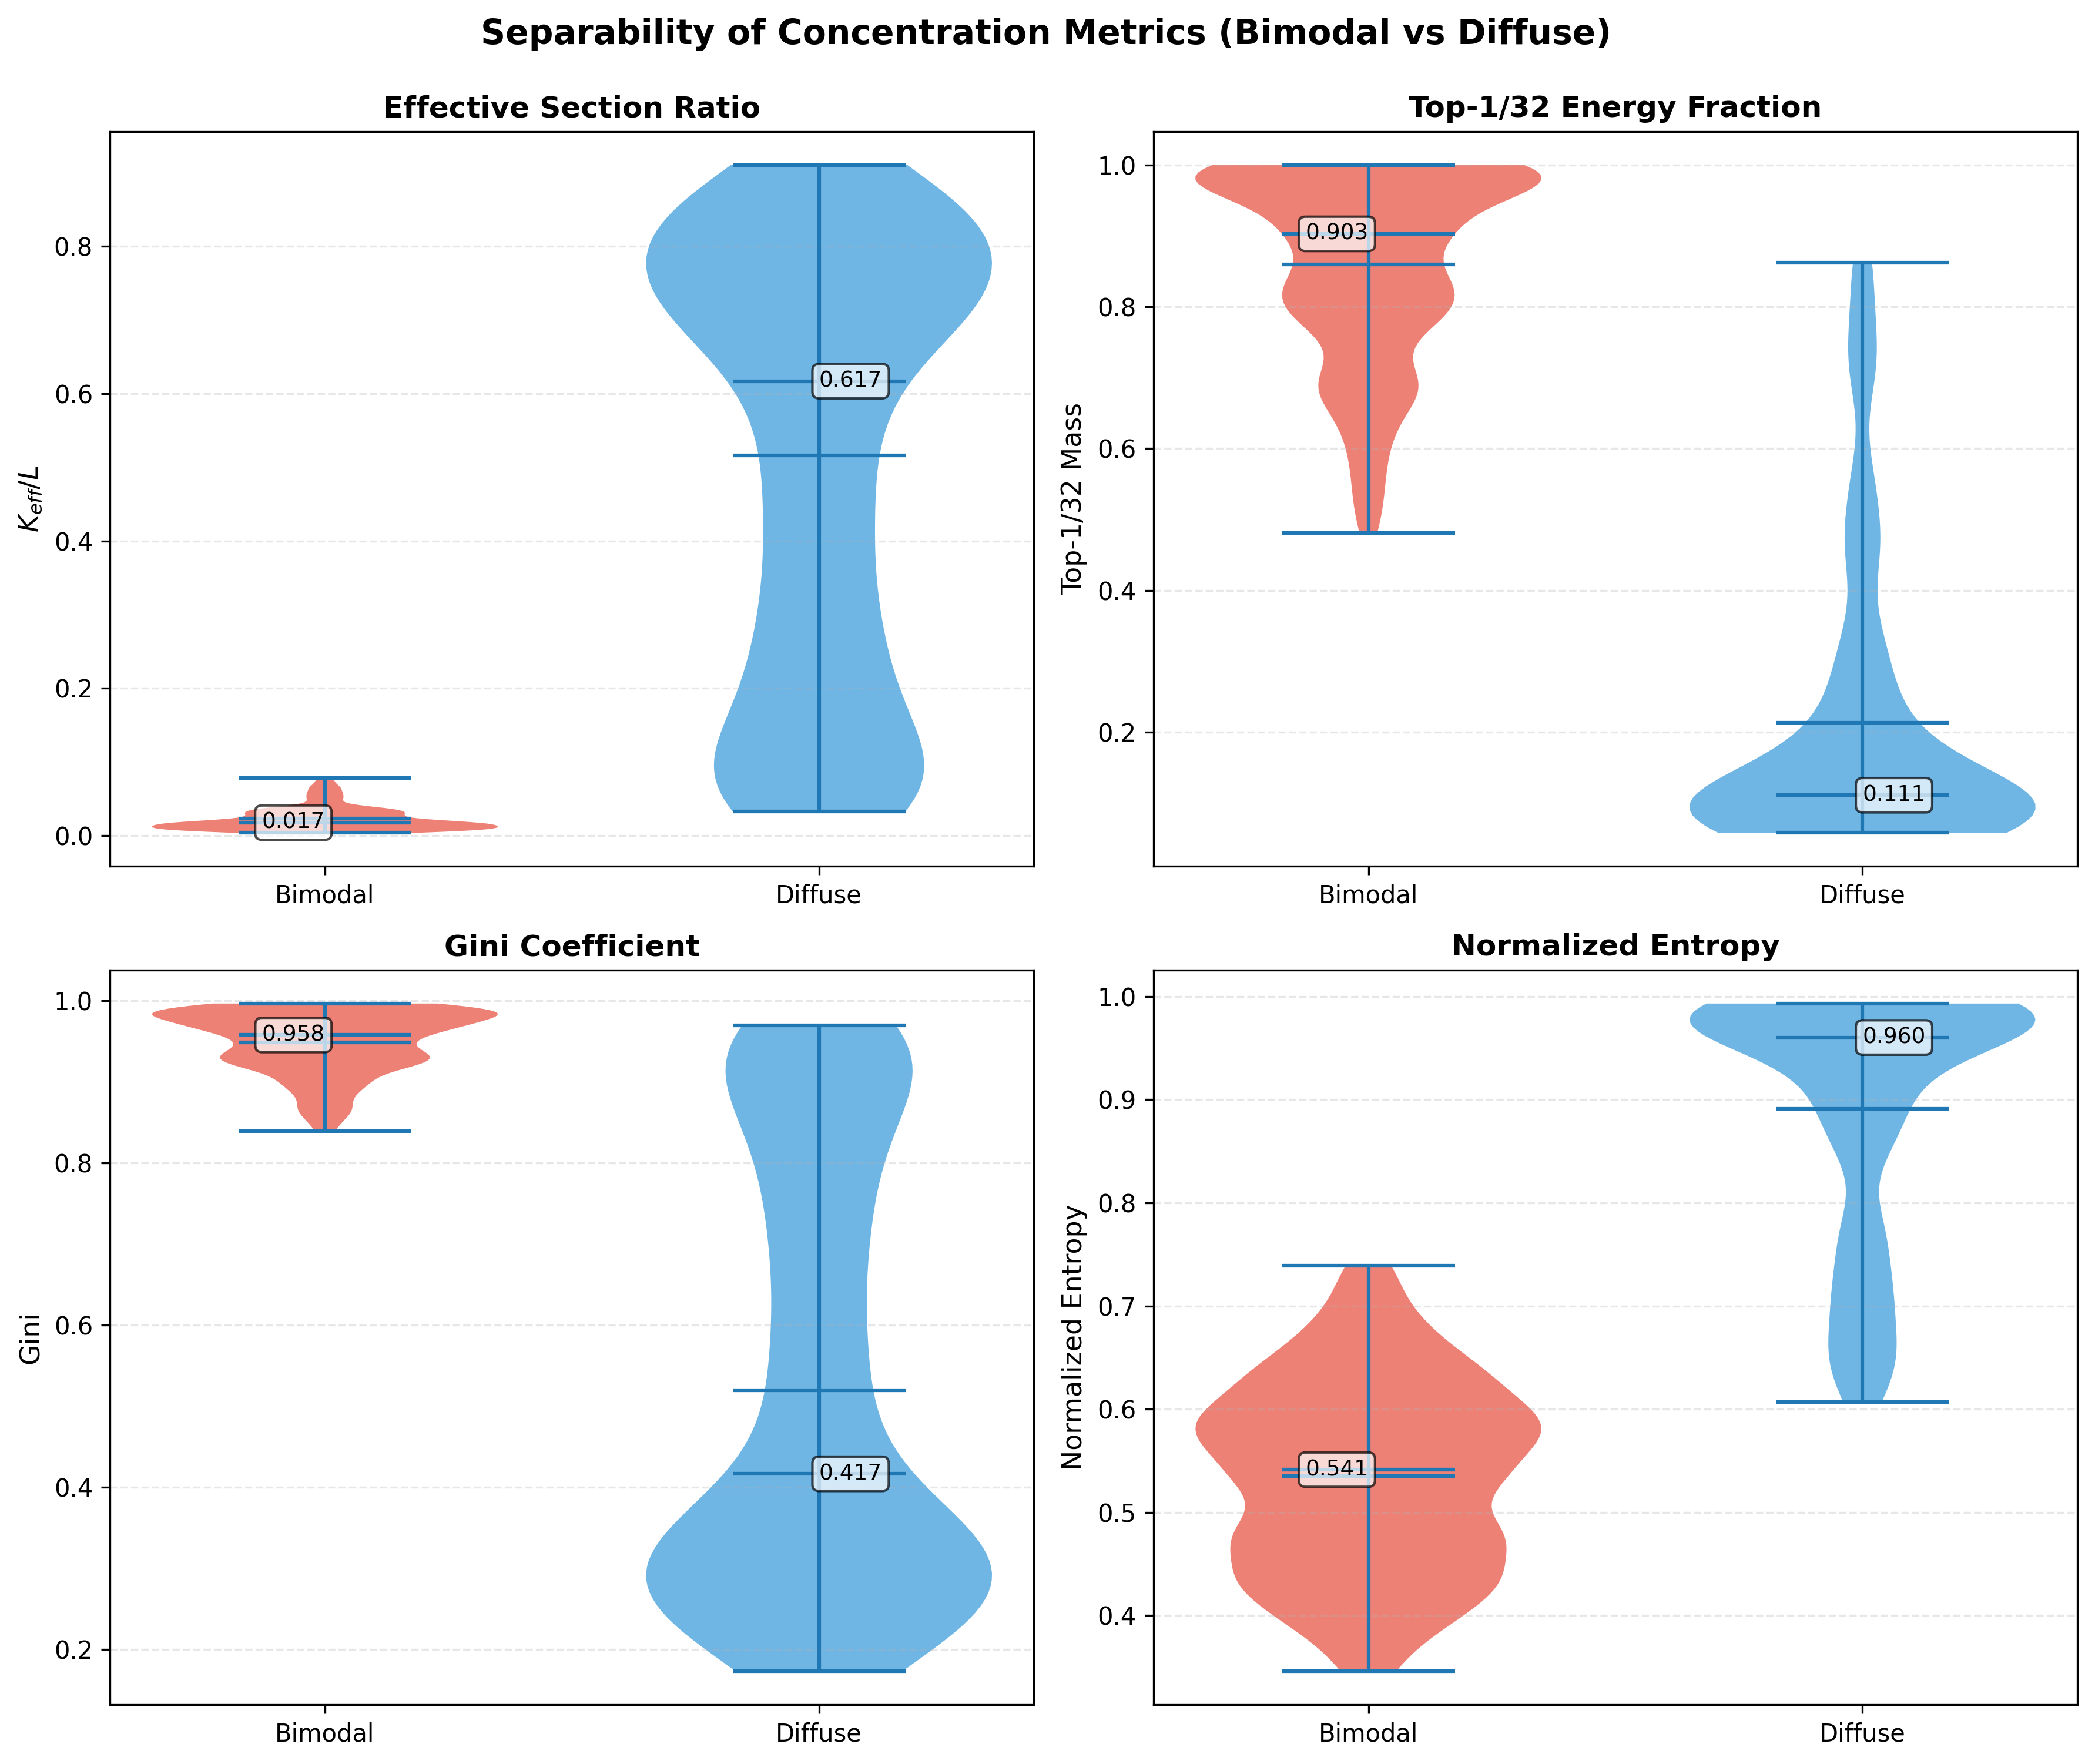
\includegraphics[width=0.9\linewidth]{figures/figure1a_separability_violin.png}
\caption{Comparison of gating metric candidates: $K_{\text{eff}}/L$ achieves the largest separation (approximately $36\times$) with the smallest distributional overlap.}
\label{fig:c3-b1}
\end{figure}

\paragraph{Semantic validity with respect to spatial extent}
Beyond separation, a concentration metric should primarily reflect how dispersed the differences are across segments, rather than being dominated by the discrepancy size $D$. To verify this property, we compared two bimodal settings: one holding total $D$ fixed and diluting each segment's differences as $B$ increases, and another holding per-segment difference $d_{\text{big}}{=}10000$ fixed so that total $D$ grows with $B$. Taking a representative slice at $L{=}2048$ (Table~\ref{tab:c3-3}), the response of $K_{\text{eff}}/L$ to $B$ is nearly identical under the two settings, indicating that the statistic's magnitude is primarily driven by $B$ (spatial extent) rather than directly by total scale $D$.

\begin{table}[!htbp]
\centering
\small
\begin{tabular}{rcc}
\toprule
$B$ & Fixed $D$ (dilution) setting & \shortstack{Fixed $d_{\text{big}}$ ($D=B\times 10^4$) \\ setting} \\
\midrule
1 & 0.0018 & 0.0018 \\
10 & 0.017 & 0.017 \\
50 & 0.078 & 0.079 \\
200 & 0.25 & 0.25 \\
\bottomrule
\end{tabular}
\caption{Response of $K_{\text{eff}}/L$ to $B$: fixed $D$ vs.\ fixed $d_{\text{big}}$.}
\label{tab:c3-3}
\end{table}


\subsection{Scale Separation and Observability Boundary}
\label{sec:appendix-gating-separation}

This section further provides a theoretical derivation of the scale separation between the two discrepancy classes, and then shows through empirical evidence how this separation degrades under low occupancy. Together, these results establish the basis for the occupancy threshold used by gating.

\paragraph{Scale separation for concentrated faults}
Let $w_s=E_s/\sum_s E_s$, $H=\sum_s w_s^2$, $K_{\text{eff}}=1/H$. Suppose there exists a hot section set $\mathcal{S}$ ($|\mathcal{S}|=S$) whose energy mass share is $\sum_{s\in\mathcal{S}}w_s=1-\varepsilon$. This paragraph expands the derivation details of $K_{\text{eff}}\le S/(1{-}\varepsilon)^2$ referenced in \S\ref{sec:eval-dedrift}. Note that:
\[
H=\sum_s w_s^2 \ge \sum_{s\in\mathcal{S}} w_s^2 \ge \frac{\left(\sum_{s\in\mathcal{S}} w_s\right)^2}{|\mathcal{S}|}=\frac{(1-\varepsilon)^2}{S},
\]
and therefore:
\[
K_{\text{eff}}=\frac{1}{\sum_s w_s^2}\le \frac{S}{(1-\varepsilon)^2}.
\]

This inequality provides an upper bound. When the energy within the hot set is approximately uniformly distributed across sections (i.e., $\varepsilon$ is small and each hot section's weight is of the same order), the bound becomes tight and $K_{\text{eff}}$ falls at the scale of $S$, so:
\[
\frac{K_{\text{eff}}}{L}=\Theta\!\left(\frac{S}{L}\right).
\]
For concentrated faults, $B$ dirty segments each cover $W$ contiguous positions on the section axis. When $B\cdot W\ll L$, the windows of different dirty segments are nearly non-overlapping on the section axis, and the total number of hot sections can be approximated as $S\approx B\cdot W$, giving $K_{\text{eff}}/L$ at the scale of $B\cdot W/L$. With typical parameters $L=2048$, $B=10$, $W=4$, the theoretical estimate is $K_{\text{eff}}/L \approx BW/L = 40/2048 \approx
0.020$; the corresponding experimental median for bimodal in \S\ref{sec:eval-dedrift} is approximately 0.017, consistent in order of magnitude. Note that when $B\cdot W$ is no longer much smaller than $L$, window overlap causes the effective number of hot sections to fall below $B\cdot
W$, and the above approximation breaks down---this is precisely the microscopic mechanism behind the capacity-axis degradation in \S\ref{sec:eval-operating}.

\paragraph{Diffuse-case scaling and observability boundary}
For diffuse differences, energy is approximately uniformly spread across the touched effective sections. Let the number of touched sections be $L_{\text{eff}} = \text{occupancy}\cdot L$, with each section's energy weight approximately equal, $w_s
\approx 1/L_{\text{eff}}$. Then $H = L_{\text{eff}} \cdot (1/L_{\text{eff}})^2 = 1/L_{\text{eff}}$, so $K_{\text{eff}} = L_{\text{eff}}$, i.e.:
\[
\frac{K_{\text{eff}}}{L}\approx \frac{L_{\text{eff}}}{L}\approx \text{occupancy}.
\]
When the occupancy of the diffuse case drops to the same order as $B\cdot W/L$, the diffuse-case $K_{\text{eff}}/L$ is compressed into the same numerical interval as the concentrated case, and threshold discrimination becomes unreliable. This marks the observability boundary of the probe: below this region, the signal no longer supports reliable shape classification, so low-occupancy samples should be excluded from such decisions.

\paragraph{Empirical manifestation of the observability boundary}
We next examine representative configurations and a broader parameter sweep to show how the diffuse-case collapse appears in practice as occupancy decreases.

\begin{table}[!htbp]
\centering
\small
\begin{tabular}{rcrr}
\toprule
$P$ & $L$ & occupancy & $K_{\text{eff}}/L$ \\
\midrule
$10^5$ & 2048 & 1.000 & 0.877 \\
$10^4$ & 4096 & 1.000 & 0.838 \\
$3\times 10^3$ & 8192 & 0.367 & 0.321 \\
$10^3$ & 4096 & 0.245 & 0.215 \\
$10^3$ & 16384 & 0.061 & 0.054 \\
$10^3$ & 32768 & 0.031 & 0.027 \\
\bottomrule
\end{tabular}
\caption{Occupancy and $K_{\text{eff}}/L$ for diffuse workloads under representative configurations. From top to bottom, occupancy decreases and $K_{\text{eff}}/L$ systematically declines, consistent with the theoretical prediction $K_{\text{eff}}/L \approx \text{occupancy}$.}
\label{tab:c3-2}
\end{table}

Table~\ref{tab:c3-2} shows a set of representative configurations covering high, medium, and low occupancy levels. In the high-occupancy region ($P{=}10^5$
or $P{=}10^4$, occupancy reaching 1.0), $K_{\text{eff}}/L$ stabilizes near 0.84--0.88, close to the theoretical upper limit. As occupancy decreases due to increasing $L$ or decreasing $P$, $K_{\text{eff}}/L$ systematically declines: when
occupancy drops to 0.061, $K_{\text{eff}}/L$ is only 0.054, already entering the numerical range that can overlap with borderline bimodal cases.

Figure~\ref{fig:c3-b2} further shows the continuous trend across multiple $(P, L)$ configurations: as occupancy decreases, $K_{\text{eff}}/L$ declines approximately linearly, consistent with the theoretical prediction $K_{\text{eff}}/L \approx \text{occupancy}$,
indicating that this is a stable structural regularity.




\begin{figure}[!htbp]
\centering
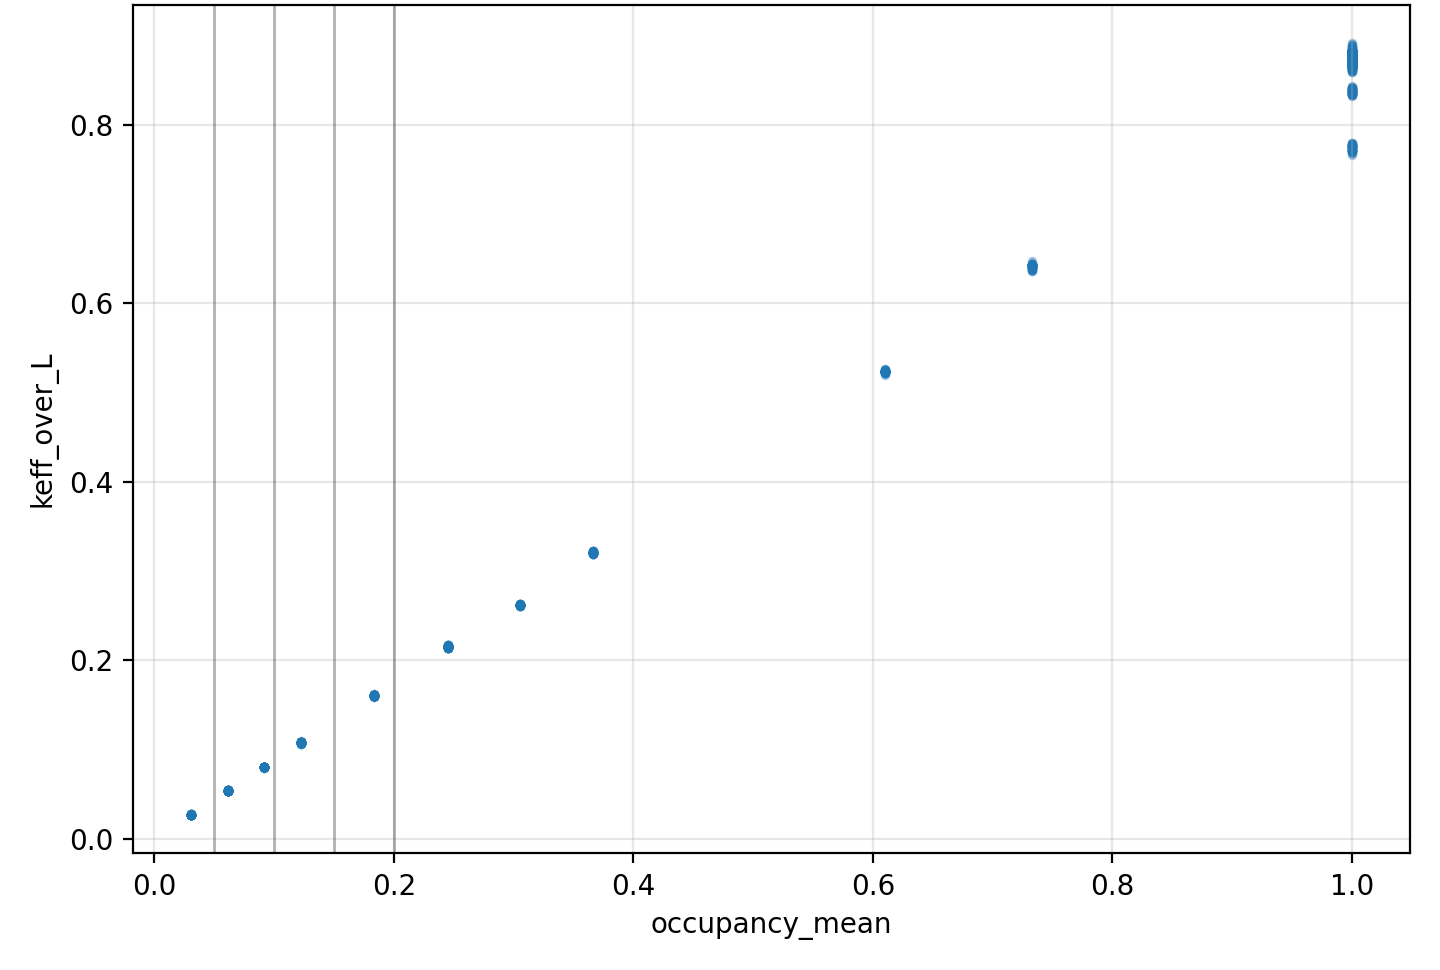
\includegraphics[width=0.9\linewidth]{figures/fig_diffuse_keff_vs_occupancy.png}
\caption{Relationship between $K_{\text{eff}}/L$ and occupancy for diffuse workloads. Each point corresponds to the aggregated result of a $(P, L)$ configuration group; on the right (high occupancy) $K_{\text{eff}}/L$ approaches the theoretical upper limit, while on the left it systematically decreases with declining occupancy.}
\label{fig:c3-b2}
\end{figure}

\subsection{Abstention Cost and Conditional Discrimination Quality}
\label{sec:appendix-gating-tristate}

\paragraph{Why unconditional discrimination has a floor}
Figure~\ref{fig:dedrift-far-frr-all} in the main text already showed the unconditional $\mathrm{FAR}$--$\mathrm{FRR}$ trade-off, where FRR has a floor determined by low-occupancy samples. This section explains this phenomenon from two angles.

When $\tau_{\text{occ}}{=}0$ (i.e., no occupancy threshold is set), all samples are forced into either bimodal or diffuse classification, and FAR and FRR cannot be simultaneously suppressed (see the corresponding curve in Figure~\ref{fig:dedrift-far-frr-all}). This degradation has two layers of causes. The first layer is statistical distortion: in low-occupancy samples, a large number of sections are never touched, and the diffuse-case $K_{\text{eff}}/L$ undergoes the structural collapse analyzed in the previous section, overlapping with the bimodal value range---this is precisely the problem that the occupancy threshold is designed to solve, and excluding these samples from classification eliminates it.

The second layer is the inherent limit of the gating task itself: taking $L{=}2048$ as an example, $B{=}200$ corresponds to a dirty segment fraction of approximately
10\%, at which point the pattern has already substantially diffused and exhibits genuine overlap with the diffuse class. Such overlap stems from the physical convergence of the two regimes in this parameter range and cannot be eliminated by raising $\tau_{\text{occ}}$; it constitutes an unavoidable ambiguity zone for gating.

\begin{table}[!htbp]
\centering
\small
\begin{tabular}{rcccc}
\toprule
$\tau_{\text{occ}}$ & \shortstack{diffuse\\classified} & \shortstack{diffuse\\\texttt{unknown}} & \shortstack{bimodal\\classified} & \shortstack{bimodal\\\texttt{unknown}} \\
\midrule
0.05 & 95.7\% & 4.3\% & 25.0\% & 75.0\% \\
0.10 & 87.0\% & 13.0\% & 8.3\% & 91.7\% \\
0.15 & 82.6\% & 17.4\% & 8.3\% & 91.7\% \\
0.20 & 78.3\% & 21.7\% & 8.3\% & 91.7\% \\
\bottomrule
\end{tabular}
\caption{Effect of different $\tau_{\text{occ}}$ on the proportion of definitive classifications vs.\ \texttt{unknown}. The proportion of definitively classified samples is defined as $\Pr(\text{occupancy}\ge\tau_{\text{occ}})$; the remaining samples output \texttt{unknown}, for which the probe withholds a shape-based recommendation and deployment policy determines the downstream action.}
\label{tab:c3-5}
\end{table}

\paragraph{Abstention cost under the occupancy threshold}
The three-state design excludes the region with insufficient occupancy from classification, trading abstention for improved discrimination quality. Table~\ref{tab:c3-5} quantifies this trade-off: taking $\tau_{\text{occ}}{=}0.10$ as an example, approximately 87\% of diffuse samples still fall within the observable region, while the majority of bimodal samples (especially those with small $B$) are excluded due to insufficient occupancy. This is operationally acceptable: low occupancy corresponds precisely to the concentrated pattern where triage is most effective, so an \texttt{unknown} verdict in this region withholds a shape recommendation rather than masking a diffuse fault. Deployment policy may choose to attempt a budget-capped triage pass informed by $\hat{D}$ and occupancy, but this decision is not driven by a shape verdict.



\paragraph{Conditional discrimination after filtering}
After the occupancy threshold filters out low-observability samples, the system computes conditional error rates only on definitively classified samples. Compared with the unconditional view in the main text (Figure~\ref{fig:dedrift-far-frr-all}), the conditional error rates can simultaneously approach 0 (Figure~\ref{fig:dedrift-far-frr-cond}).

Because the workload configurations form a discrete grid, each
$(\tau_{\text{occ}}, \tau_{\text{gating}})$ pair yields a
single $(\mathrm{FAR}, \mathrm{FRR})$ point rather than a
continuous curve. Dominated points---those for which another
threshold setting achieves both lower FAR and lower FRR---carry
no decision-relevant information and are omitted; the retained
non-dominated frontier (Pareto front) is a standard
presentation for discrete multi-objective trade-offs. Dashed
lines serve as visual guides only.

\begin{figure}[!htbp]
\centering
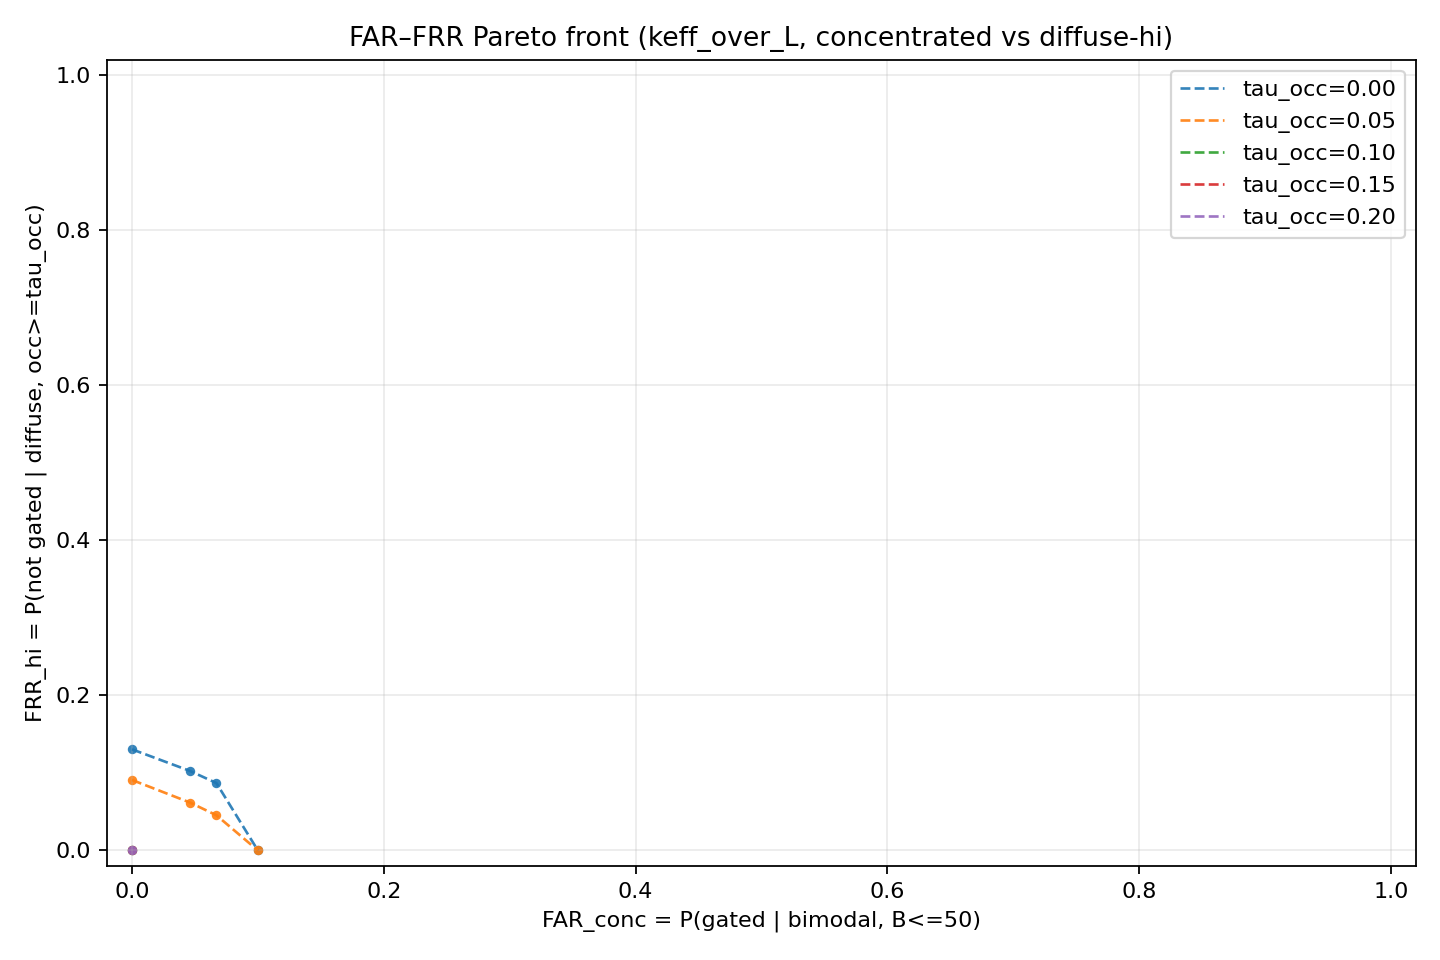
\includegraphics[width=0.9\linewidth]{figures/fig_far_frr_conc_vs_diffuse_hi_pareto.png}
\caption{Conditional $\mathrm{FAR_{cond}}$--$\mathrm{FRR_{cond}}$ trade-off on definitively classified samples (read in the same way as Figure~\ref{fig:dedrift-far-frr-all}). FAR is computed only on concentrated workloads with $B \le 50$ (excluding $B{=}200$, whose pattern has already converged toward diffuse); FRR is computed only on diffuse samples with $\text{occupancy} \ge \tau_{\text{occ}}$. When $\tau_{\text{occ}} \geq 0.10$, both error rates simultaneously approach 0.}
\label{fig:dedrift-far-frr-cond}
\end{figure}
